\section*{Schaltungssimulationen in LTSpice, Aufgabe 2.2}\label{sec:ag2.2}
Der in Aufgabe 2.1 vorgestellte harmonische Oszillator soll nun mit Hilfe des Programms \glqq LT-Spice\grqq{} zur Simulation elektrischer Schaltungen nachgebaut und berechnet werden. Da es keine Strom- bzw. Spannungsquelle in der Schaltung gibt, wird am Kondensator eine initiale Spannung zum Zeitpunkt $t = 0$ von 12\volt angelegt. Es handelt sich um eine transiente Simulation, also eine Simulation, bei der zeitabhängige Einflüsse berücksichtigt werden. Der Simulationsbereich bewegt sich zwischen $0$ und $25$ \si{\milli\second}. \\
Die in LT-Spice erzeugte Schaltung wird nun mit der analytisch berechneten Funktion aus Aufgabenteil 1 verglichen. Hierzu sind an verschieden Zeitpunkten $t$ , $t \in [0,25]$ \si{\milli\second} Stromwerte aus dem Graphen in LT-Spice abgelesen worden, sowie die Werte mit Hilfe der Funktion zu gleichen Zeitpunkt $t$ händisch berechnet worden.\\ \\
Daraus ergibt sich die folgende Tabelle\\ \\
\begin{table}[h]
	\centering
	\begin{tabular}[h]{c|c|c}
		Zeitpunkt $t$ in \si{\milli\second} & LT-Spice Wert in \si{\milli\ampere} \ & Berechneter Wert in \si{\milli\ampere} \\
		\hline
		1 & -487,18 & -494,26 \\
		2 & -159,73 & -149,67\\
		3 & 102,45 & 110,23\\
		6 & -28,39 & -28,46\\
		9 & 4,57 & 3,91\\
		12 & -0,356 & -0,122\\
		15 & -0,048 & -0,090\\
	\end{tabular}
\end{table}\\
\\

Zusätzlich zu den Messwerten wurde der Graph der Funktion aus Aufgabenteil 2.1 in Matlab geplottet. Vergleich man nun sowohl die Funktionswerte in der Tabelle, als auch die beiden entstandenen Graphen \ref{lt} und \ref{mat} , so wird deutlich, dass die Funktion aus 2.1 den gleichen Graphen erzeugt wie die Simulation in LT-Spice. Außerdem ist zu erkennen, dass die Amplitude bei fortlaufender Zeit kleiner wird und der Strom gegen $0\:$\si{\milli\ampere} konvergiert. Die Unterschiede in den Funktionswerten der Tabelle lassen sich auf Rundungsfehler, sowie Ablesefehler in LT-Spice zurückführen.
\begin{figure}[h]
	\centering
	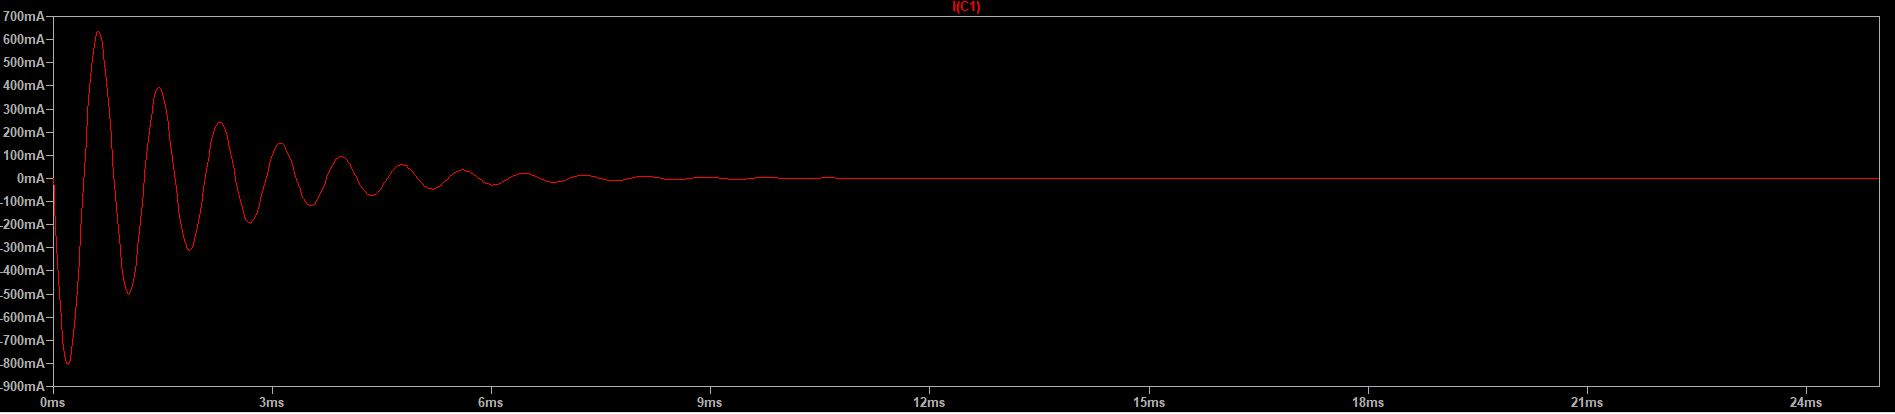
\includegraphics[width=\textwidth]{data/ltsim}
	\caption{Simulationsgraph aus LT-Spice}
	\label{lt}
\end{figure}

\begin{figure}[h!]
	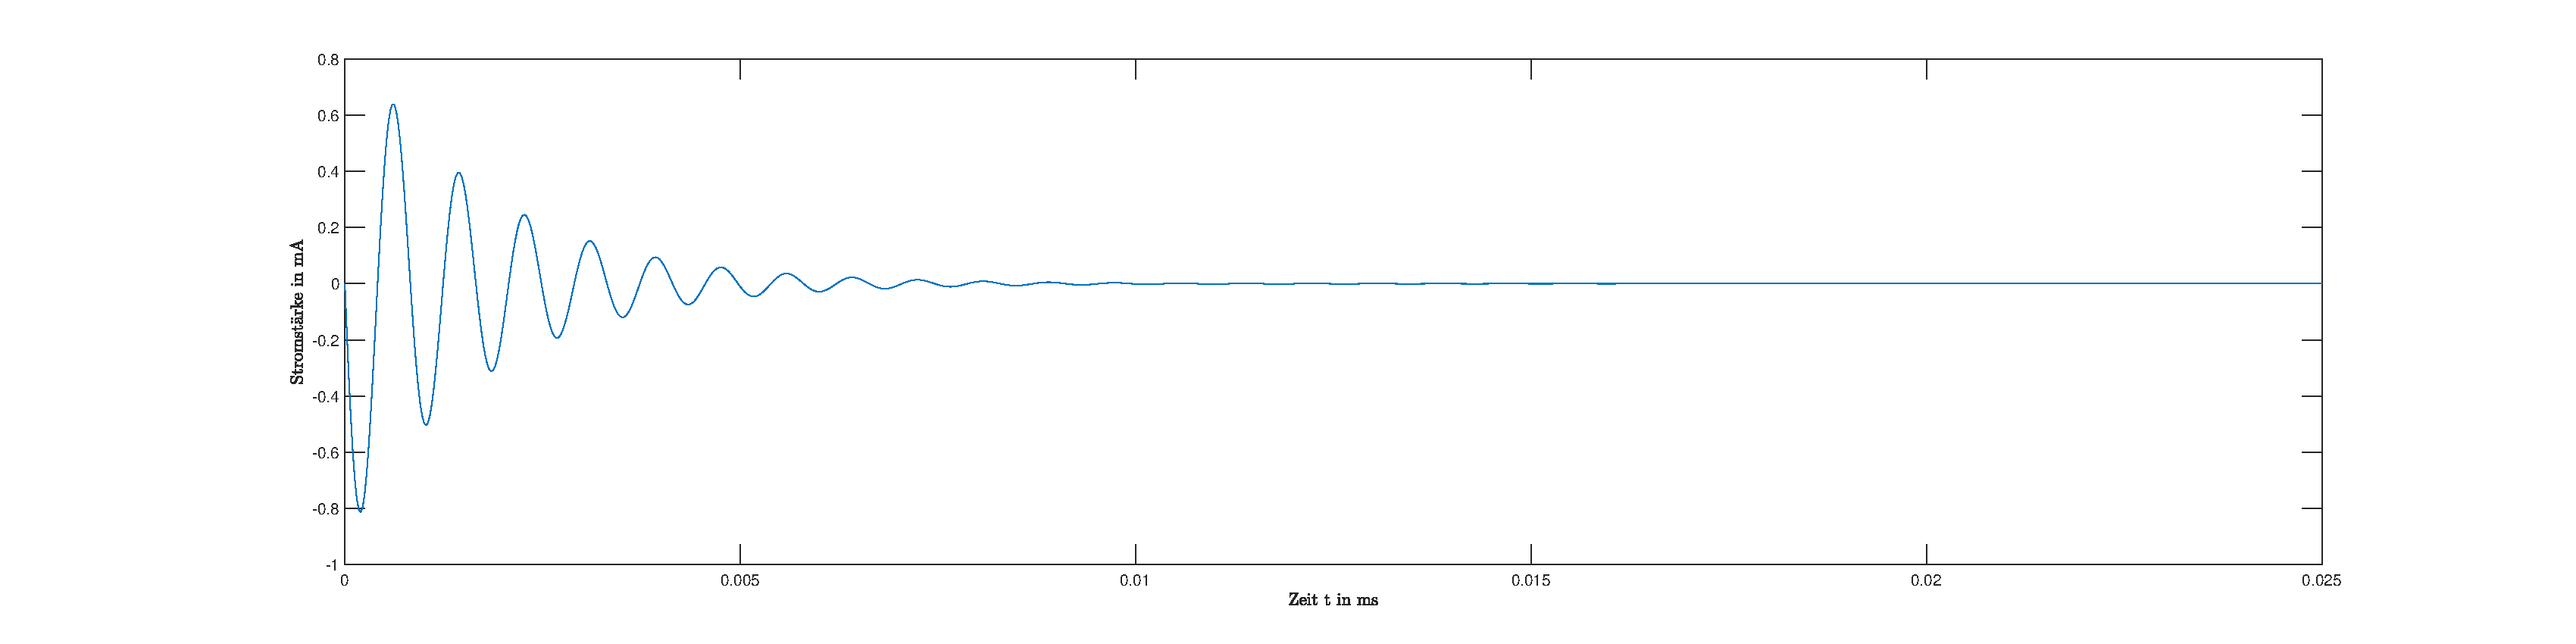
\includegraphics[width=\textwidth]{data/fctmat}
	\caption{Simulationsgraph aus Matlab}
	\label{mat}
\end{figure}
\newpage
Des Weiteren soll untersucht werden, inwiefern sich ein kleinerer Widerstand $R$ auf den Funktionsgraphen auswirkt. Hierzu wurde der Widerstand $R$ in dem harmonischen Oszillator auf den Wert $0,5\:$\si{\ohm} gesetzt. Aus der Graphik \ref{14R} geht hervor, dass die Amplituden durch einen kleineres $R$ beeinträchtigt wird. Wegen der verkleinerten Widerstand nimmt die Auslenkung langsamer ab, gleichzeitig ist der maximal fließende Strom,  höher als der Maximalstrom bei einem größeren Widerstand. Die Periodendauer bleibt unbeeinträchtigt.
\\ \\
\begin{figure}[h]
	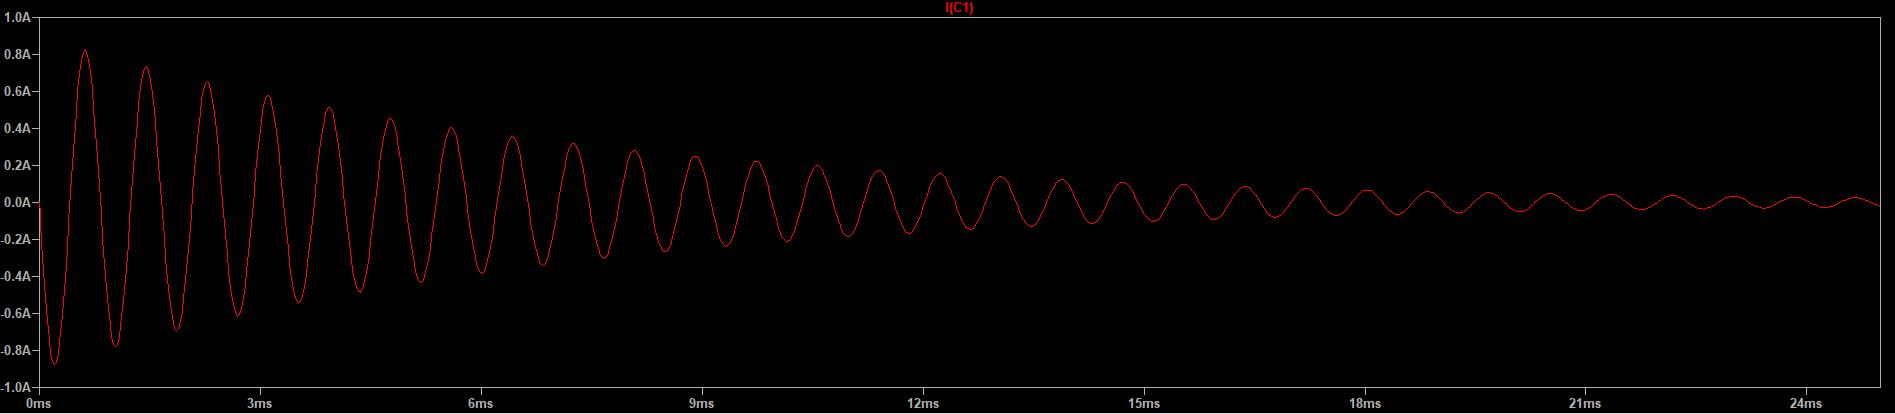
\includegraphics[width=\textwidth]{data/kleineresR}
	\caption{harmonischer Oszillator mit $R = 0,5\:$\ohm}
	\label{14R}
\end{figure}

Neben dem harmonischen Oszillator wird eine weitere Schaltung in LT-Spice betrachtet. Bei dieser Schaltung handelt es sich um einen Spannungsverdoppler. Diese ist auch unter dem Namen Villard-Schaltung bekannt.\\

Wie der Name besagt, ist das Ziel der Schaltung die Ausgangsspannung, im Vergleich zur Eingangsspannung, zu verdoppeln. Bei der gegebenen Schaltung \ref{bspS} handelt es sich nicht um einen Standard Spannungsverdoppler, der nur aus einer Diode und einem Kondensator besteht, sondern um einen von Greinacher erweiterten Spannungsverdoppler . Bei diesem ist der Villard-Schaltung, die aus dem Kondensator C1 und der Diode D1 besteht, noch ein Kondensator C2 und eine Diode D2 nachgeschaltet. Zusätzlich wurde der Widerstand R1 in Reihe zur Spannungsquelle geschaltet. Voraussetzung für Villard-Schaltung ist eine Quelle, die eine Wechselspannung erzeugt. \\

\begin{figure}[h!]
	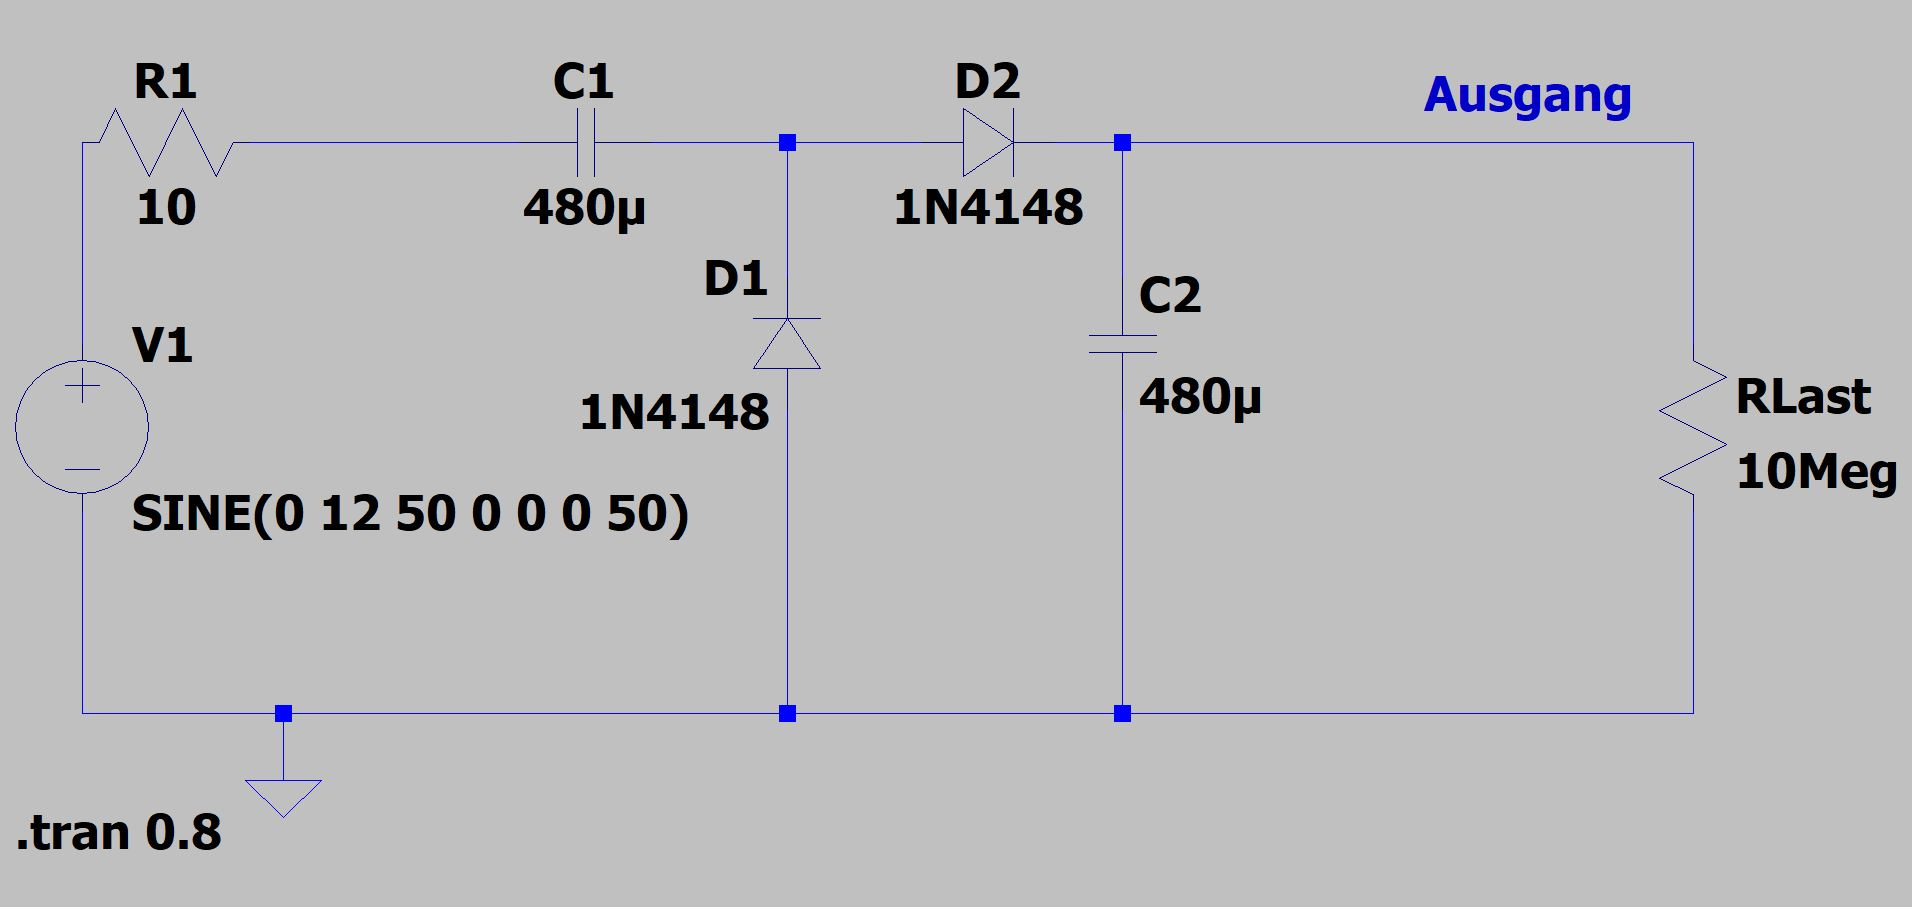
\includegraphics[width=\textwidth]{data/bspschaltung}
	\caption{Spannungsverdoppler}
	\label{bspS}
\end{figure}

\newpage

Der Kondensator C1 wird während der ersten positiven Halbperiode auf die Eingangsspannung, also die Spannung $u_{e}$, aufgeladen. In der darauf folgenden negativen Halbperiode findet nun ein Ladungsaustausch zwischen der Kondensatoren C1 und C2 statt. Die Diode D1 schließt sich und die Diode D2 öffnet sich. Dadurch fließt ein Strom über C2 zurück zur Spannungsquelle. C1 wird hierbei entladen und lädt den Kondensator C2 auf. Die Spannung an C2 beträgt am Ende der Periode den Wert der Eingangsspannung $u_{e}$. \\
Bei der nächsten positiven Halbperiode wird der Kondensator C1 wieder auf die Eingangspannung geladen, beim Wechsel zur negativen Halbperiode wird C1 auf die halbe Spannung entladen, C2 jedoch auf den 1,5-fachen Wert. Dies führt sich so weiter fort, bis die Spannung an C2 den doppelten Wert der Eingangsspannung erreicht hat.
\\ \\
Der doppelte Wert der Eingangsspannung wird nicht erreicht, da der Spannungsabfall bei einer Silizium Diode ca. $0,7\:$\si{\volt} beträgt. In der gegeben Schaltung sind zwei Dioden verbaut, deshalb liegt der Spannungsabfall bei ca. $1,4\:$\si{\volt}. 
\\ \\ 
Vergrößert man bei der Schaltung den Ladewiderstand, so beobachtet man in der Abbildung \ref{grossEin}, dass die Spannung am Ausgang bzw. am Kondensator C2 langsamer steigt.Dies ist dadurch zu begründen, dass durch den erhöhten Ladewiderstand ein geringerer Stromfluss möglich ist und damit der Ladungsausgleich verlangsamt wird. Durch die Verkleinerung des Lastwiderstands R2 kommt es bei der negativen Halbperiode auch zu einem Spannungsabfall am Kondensator C2, siehe Abbildung \ref{kleinLast}. Die Auswirkungen eines kleinen Lastwiderstandes mit großem Ladewiderstand sind in Abbildung \ref{fig:groKlein} graphisch dargestellt.

\begin{figure}
	\centering
	\begin{subfigure}[b]{\textwidth}
		\centering
		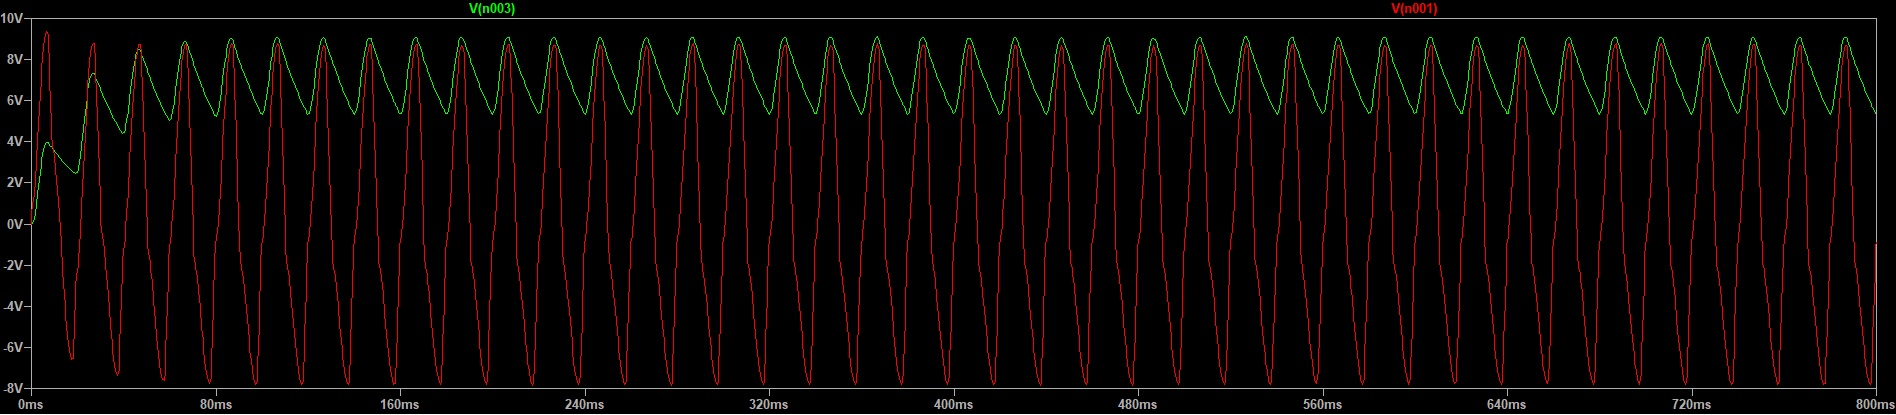
\includegraphics[width=\textwidth]{data/kleinLast}
		\caption{Spannungsverlauf bei kleinem Lastwiderstand}
		\label{kleinLast}
	\end{subfigure}
	\begin{subfigure}[b]{\textwidth}
		\centering
		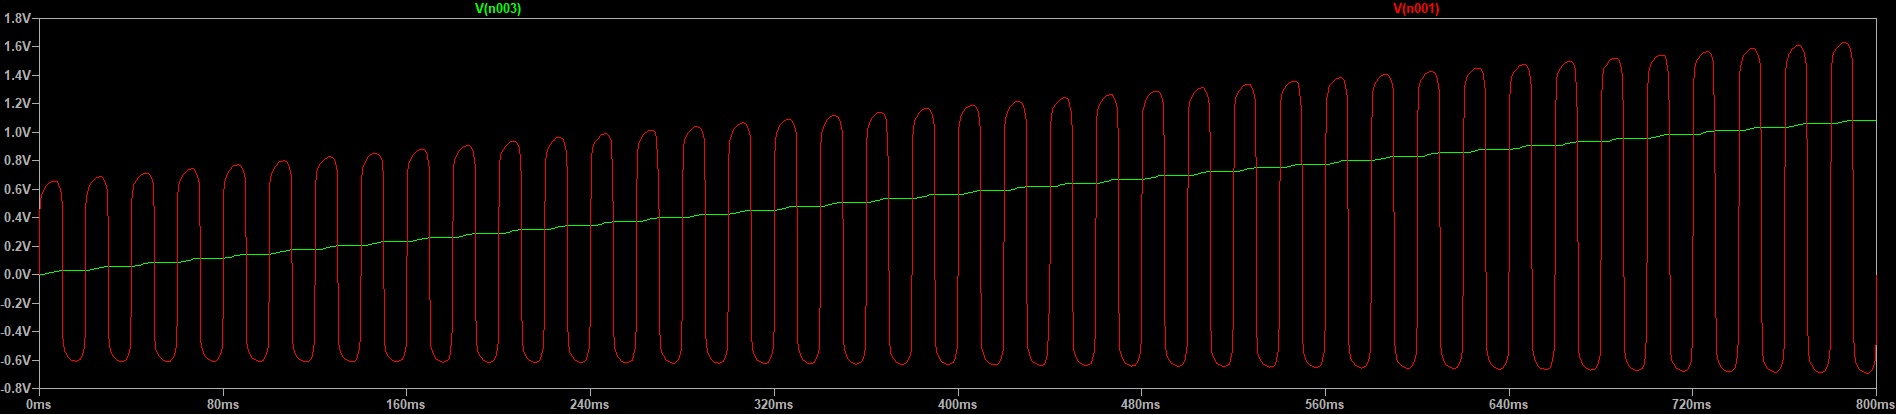
\includegraphics[width=\textwidth]{data/grossEin}
		\caption{Spannungsverlauf bei großem Ladewiderstand}
		\label{grossEin}
	\end{subfigure}
	\begin{subfigure}[b]{\textwidth}
		\centering
		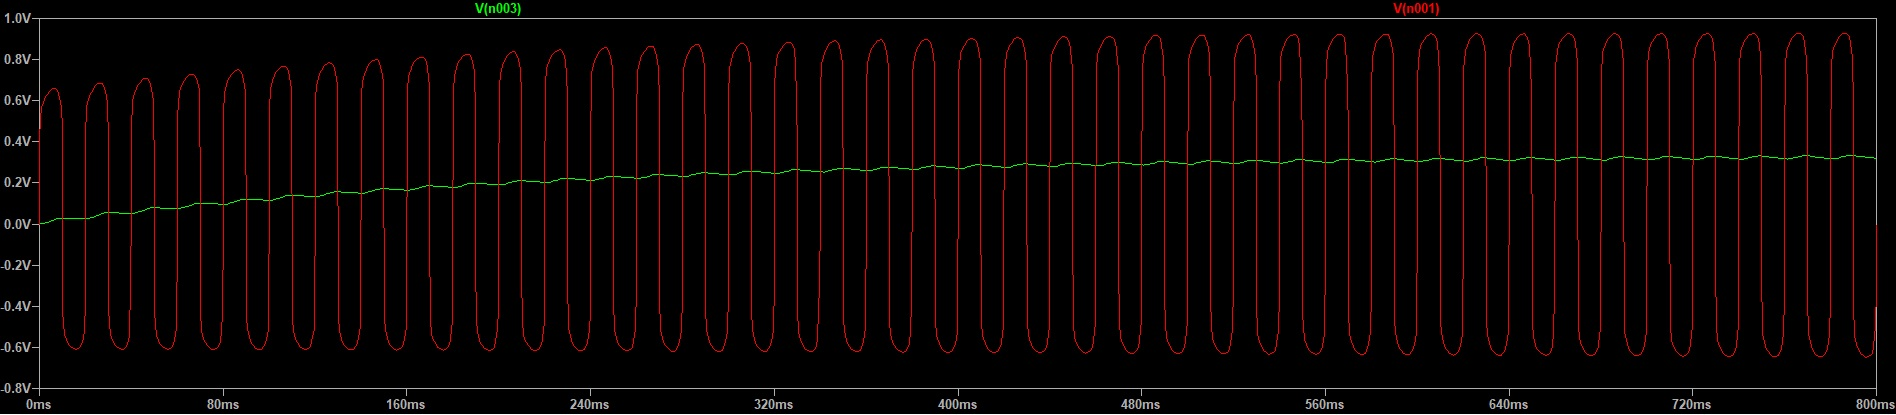
\includegraphics[width=\textwidth]{data/grossEin_kleinLast}
		\caption{Spannungsverlauf bei kleinem Lastwiderstand und großem Ladewiderstand}
		\label{fig:groKlein}
	\end{subfigure}
\caption{Verschiedene Spannungsverläufe, rot ist Spannung hinter dem Widerstand, grün die Ausgangsspannung}
\end{figure}